
% Template for Elsevier CRC journal article
% version 1.2 dated 09 May 2011

% This file (c) 2009-2011 Elsevier Ltd.  Modifications may be freely made,
% provided the edited file is saved under a different name

% This file contains modifications for Procedia Computer Science

% Changes since version 1.1
% - added "procedia" option compliant with ecrc.sty version 1.2a
%   (makes the layout approximately the same as the Word CRC template)
% - added example for generating copyright line in abstract

%-----------------------------------------------------------------------------------

%% This template uses the elsarticle.cls document class and the extension package ecrc.sty
%% For full documentation on usage of elsarticle.cls, consult the documentation "elsdoc.pdf"
%% Further resources available at http://www.elsevier.com/latex

%-----------------------------------------------------------------------------------

%%%%%%%%%%%%%%%%%%%%%%%%%%%%%%%%%%%%%%%%%%%%%%%%%%%%%%%%%%%%%%
%%%%%%%%%%%%%%%%%%%%%%%%%%%%%%%%%%%%%%%%%%%%%%%%%%%%%%%%%%%%%%
%%                                                          %%
%% Important note on usage                                  %%
%% -----------------------                                  %%
%% This file should normally be compiled with PDFLaTeX      %%
%% Using standard LaTeX should work but may produce clashes %%
%%                                                          %%
%%%%%%%%%%%%%%%%%%%%%%%%%%%%%%%%%%%%%%%%%%%%%%%%%%%%%%%%%%%%%%
%%%%%%%%%%%%%%%%%%%%%%%%%%%%%%%%%%%%%%%%%%%%%%%%%%%%%%%%%%%%%%

%% The '3p' and 'times' class options of elsarticle are used for Elsevier CRC
%% The 'procedia' option causes ecrc to approximate to the Word template
\documentclass[3p,times,procedia]{elsarticle}
\flushbottom

%% The `ecrc' package must be called to make the CRC functionality available
\usepackage{ecrc}
\usepackage{multirow}
\usepackage{comment}
%\usepackage{amsmath}


%% The ecrc package defines commands needed for running heads and logos.
%% For running heads, you can set the journal name, the volume, the starting page and the authors

%% set the volume if you know. Otherwise `00'
\volume{00}

%% set the starting page if not 1
\firstpage{1}

%% Give the name of the journal
\journalname{Procedia Computer Science}

%% Give the author list to appear in the running head
%% Example \runauth{C.V. Radhakrishnan et al.}
\runauth{A. Karapetyan, W. Yaqub et al.}

%% The choice of journal logo is determined by the \jid and \jnltitlelogo commands.
%% A user-supplied logo with the name <\jid>logo.pdf will be inserted if present.
%% e.g. if \jid{yspmi} the system will look for a file yspmilogo.pdf
%% Otherwise the content of \jnltitlelogo will be set between horizontal lines as a default logo

%% Give the abbreviation of the Journal.
\jid{procs}

%% Give a short journal name for the dummy logo (if needed)
%\jnltitlelogo{Procedia Computer Science}

%% Hereafter the template follows `elsarticle'.
%% For more details see the existing template files elsarticle-template-harv.tex and elsarticle-template-num.tex.

%% Elsevier CRC generally uses a numbered reference style
%% For this, the conventions of elsarticle-template-num.tex should be followed (included below)
%% If using BibTeX, use the style file elsarticle-num.bst

%% End of ecrc-specific commands
%%%%%%%%%%%%%%%%%%%%%%%%%%%%%%%%%%%%%%%%%%%%%%%%%%%%%%%%%%%%%%%%%%%%%%%%%%

%% The amssymb package provides various useful mathematical symbols

\usepackage{amssymb}
%% The amsthm package provides extended theorem environments
%% \usepackage{amsthm}

%% The lineno packages adds line numbers. Start line numbering with
%% \begin{linenumbers}, end it with \end{linenumbers}. Or switch it on
%% for the whole article with \linenumbers after \end{frontmatter}.
%% \usepackage{lineno}

%% natbib.sty is loaded by default. However, natbib options can be
%% provided with \biboptions{...} command. Following options are
%% valid:

%%   round  -  round parentheses are used (default)
%%   square -  square brackets are used   [option]
%%   curly  -  curly braces are used      {option}
%%   angle  -  angle brackets are used    <option>
%%   semicolon  -  multiple citations separated by semi-colon
%%   colon  - same as semicolon, an earlier confusion
%%   comma  -  separated by comma
%%   numbers-  selects numerical citations
%%   super  -  numerical citations as superscripts
%%   sort   -  sorts multiple citations according to order in ref. list
%%   sort&compress   -  like sort, but also compresses numerical citations
%%   compress - compresses without sorting
%%
%\biboptions{sort&compress}

% \biboptions{}

% if you have landscape tables
\usepackage[figuresright]{rotating}
%\usepackage{harvard}
% put your own definitions here:x
%   \newcommand{\cZ}{\cal{Z}}
%   \newtheorem{def}{Definition}[section]
%   ...

% add words to TeX's hyphenation exception list
%\hyphenation{author another created financial paper re-commend-ed Post-Script}

% declarations for front matter

\begin{document}

\begin{frontmatter}

%% Title, authors and addresses

%% use the tnoteref command within \title for footnotes;
%% use the tnotetext command for the associated footnote;
%% use the fnref command within \author or \address for footnotes;
%% use the fntext command for the associated footnote;
%% use the corref command within \author for corresponding author footnotes;
%% use the cortext command for the associated footnote;
%% use the ead command for the email address,
%% and the form \ead[url] for the home page:
%%
%% \title{Title\tnoteref{label1}}
%% \tnotetext[label1]{}
%% \author{Name\corref{cor1}\fnref{label2}}
%% \ead{email address}
%% \ead[url]{home page}
%% \fntext[label2]{}
%% \cortext[cor1]{}
%% \address{Address\fnref{label3}}
%% \fntext[label3]{}

\dochead{6th International Conference on Ambient Systems, Networks and Technologies, ANT 2015 and the 5th International Conference on Sustainable Energy Information Technology, SEIT 2015}
%% Use \dochead if there is an article header, e.g. \dochead{Short communication}
%% \dochead can also be used to include a conference title, if directed by the editors
%% e.g. \dochead{17th International Conference on Dynamical Processes in Excited States of Solids}

\title{A Two-Stage Comparative Life Cycle Assessment of Paper-Based and Software-Based Business Cards}

%% use optional labels to link authors explicitly to addresses:
%% \author[label1,label2]{<author name>}
%% \address[label1]{<address>}
%% \address[label2]{<address>}


\author[a]{Areg Karapetyan \corref{cor1}}
\ead{akarapetyan@masdar.ac.ae}
\author[a]{Waheeb Yaqub \corref{cor1}}
\ead{wyaqub@masdar.ac.ae}
\author[a]{Aram Kirakosyan}
\ead{akirakosyan@masdar.ac.ae}
\author[b]{Sgouris Sgouridis}
\ead{ssgouridis@masdar.ac.ae}

\address[a]{Department of Electrical Engineering and Computer Science, Masdar Institute of Science and Technology, Abu Dhabi, UAE}
\address[b]{Engineering Systems and Management Department, Masdar Institute of Science and Technology, Abu Dhabi, UAE}



\begin{abstract}
%% Text of abstract
We conduct a comparative life cycle assessment of two business card options: a smartphone software and the common paper-based alternative. Life cycle impacts of production, distribution and use of business cards were compared and contrasted for both systems. Given the prevalence and multifunctionality of digital devices and services, we analyze the environmental impacts of the two systems and evaluate their total energy consumption, Greenhouse Gas (GHG) emissions and toxic releases by conducting a two-stage life cycle assessment with alternating functional units. The results indicate that, for a small-scale functional unit, the paper-based business card system causes slightly less environmental impact and has lower energy demand than the software-based (digital) business card system. Whereas when considering the more likely, large scale (real world scenario) functional unit, the digital business card system is more environmentally friendly and economical in terms of energy consumption. By comparing these two systems, this paper serves businesses and consumers when considering environmental consequences and energy depletion of their business networking options.
\end{abstract}


\begin{keyword}
Life Cycle Assessment; Information and Communication Technologies; Software Life Cycle Assessment; Environmental Impact; Input-Output Life Cycle Assessment; Printed Business Cards; Digital Business Cards; 

%% keywords here, in the form: keyword \sep keyword

%% PACS codes here, in the form: \PACS code \sep code

%% MSC codes here, in the form: \MSC code \sep code
%% or \MSC[2008] code \sep code (2000 is the default)

\end{keyword}
\cortext[cor1]{Corresponding author. Tel.: +971-56-953-6068, +971-55-345-7753 }
\end{frontmatter}

%\correspondingauthor[*]{Corresponding author. Tel.: +0-000-000-0000 ; fax: +0-000-000-0000.}
%\email{akarapetyan@masdar.ac.ae, wyaqub@masdar.ac.ae }

%%
%% Start line numbering here if you want
%%
% \linenumbers

%% main text

%\enlargethispage{-7mm}
\section{Introduction}
\begin{comment}
Anthropogenic impacts on climate, natural resource depletion, industrial pollution have drawn global consciousness to the concepts of sustainability, and made it applicable not only in large-scale  industrial and commercial sectors, but also in routine activities.\\
\end{comment}
The rapid growth of the Internet and advances in digital technologies allowed the information and communication technologies (ICT) sector to revolutionize business operations with a transition from paper to digital based systems. Nowadays, paper based products and services such as billing systems, books, magazines and newspapers, diaries, business cards and office documentation all have their digital alternatives. We perform a two-stage cradle-to-grave LCA analysis to compare paper-based (PBC) and digital business card (DBC) systems in terms of their environmental impacts and energy utilization based on a comprehensive investigation of life cycle burdens of the two systems.\\

Comparative analysis of the environmental impacts of traditional paper based products and their corresponding ICT enabled digital counterparts has been a subject of a considerable body of research. These studies include but are not limited to comparison of digital and paper media, electronic and paper billing methods, printed and electronic teaching aids, e-mail and traditional postal mail service, as well as printed scholarly books and e-book reading devices \cite{Bull201410, 6360455, enroth2009, zurkirch2000, kozak2003,hischier2003m}. Business cards, cards bearing business information about a company or individual intended for networking a person or business, enjoy wide usage. According to a CNN report and a number of Internet resources, in 2012 the annual number of printed business cards was estimated to be 10 billion \cite{cnnreport}. Despite, to the best of our knowledge, no comparison between the PBC and DBC options is publicly available. PBC refers to a white or full color paper stock having printed text and/or image(s) representing information about a business or a person. Likewise, DBC refers to a digital data containing information regarding a business or a person stored in a local storage of a smartphone and accessible as a visualization. \\


Various research studies indicate that the ICT sector has enough potential for reducing global energy and resource consumption and GHG emissions  \cite{10046363,924525, 6360455}. Further modified ICT applications could save up to 7.8 GtCO2e, or 15\% of global CO2 equivalent emissions by 2020 \cite{s3758490, 7282419}. Notwithstanding, the ICT sector itself challenges the environment and global energy reserves and can cause undesirable effects on the environment  \cite{Hilty20061618, 6083606, Bull201410}. A typical Google search performed from a desktop computer can produce about 7g of CO2 per search \cite{7282419}. Considering that there are 3.5 billion Google searches per day on average, the resulting aggregate CO2 emissions only from this activity amounts to 24.5 KtCO2 per day, which is equivalent to the emissions from 2 million efficient cars (at 120 gCO2/km) driving for 100km. In 2002, the ICT sector's total contribution to global GHG emissions was estimated to be 530 MtCO2e, whereas in 2007, the emissions increased to 620 MtCO2e (17\% increase) and constituted 1.3\% of the cumulative global GHG emissions with forecasts for 2020 in the order of 1.43 GtCO2e  \cite{malmodin2013future, s3758490}. 
\begin{comment}
Quantifying and evaluating the direct environmental footprint of ICT applications is of crucial importance in terms of environmental preservation.
 Life Cycle Assessment (LCA), a widely used methodology for evaluating the environmental effects of a product or activity holistically, is discussed in the proceeding section. 
According to ISO 14040 standard ``an LCA study analyzes the environmental aspects and potential environmental impacts throughout a product's life cycle, that is, from raw material acquisition through production, use, end-of-life treatment, recycling and final disposal (i.e. cradle-to-grave) of the product'' \cite{ISO140402006}.
\end{comment}

\section{Background and Related Work} 

ISO LCA\cite{ISO140402006}, Environmental Product Declarations (EPD)\cite{iso2006environmental} and PAS 2050 \cite{pas20082050} are accepted methods for environmental impact assessment. Even though EPD provides with inclusive environmental impact evaluation tool that also identifies enhancement prospects, it overlooks certain problems such as carbon storage and the end-of-life phase. Unlike ISO LCA, PAS 2050 standards take into account only total GHG emissions, which makes this technique inflexible when conducting a comprehensive environmental impact assessment. ISO LCA is widely accepted and possesses capabilities to assess various environmental impacts of products and services \cite{cooper2006life} and ISO 14000 family is the international standard document on LCA \cite{finkbeiner201340s}.\\

Although LCA has promising capabilities, it has weaknesses and limitations with its methodological framework \cite{joshi1999product, reap2008survey, hermann2007assessing}. Uncertainty in LCA analysis could be mainly due to the input data factors such as quality, quantity, comprehensiveness, oldness  and site specificness \cite{curran2005international, reap2008survey} and is dependent on the boundary definition \cite{joshi1999product}. For products and systems that have unambiguous and straightforward interpretation or are distinct substitutes,  LCA  is effective. It is argued that this may not be the case for paper-based and  corresponding  digital  alternative products \cite{Bull201410, reap2008survey}, because of the multifunctionality of ICT systems, unpredictability of digital product usage, and the  data  scarcity \cite{Bull201410, farrant2012environmental, enroth2009}. In order to avoid the problem of allocation and multifunctionality of the studied ICT products some non-comparative ICT LCA allocate or divide the system based on functionality or based on processes (non-physical division) \cite{choi2006life,frey2006ecological}. An LCA case study for email \cite{farrant2012environmental}, included ICT equipment manufacturing in the system boundaries and concluded that production of ICT equipment is one of the most significant contributors to the environmental impact of the system. To further underline the boundary conditions' effect on the final outcome of the LCA study, a study on printed and electronic scholarly articles showed that, either printed or electronic scholarly journals were preferable, depending on the assigned boundary conditions \cite{gard2002digital}.\\

Surprisingly, while environmental impact of the hardware production, usage and disposal of ICT products has been broadly considered by a plenty of LCA research studies \cite{Bull201410, farrant2012environmental, enroth2009}, environmental aspects caused by software development attracted only limited research \cite{Moshnyaga:2013}. Similarly, the environmental impact of ICT devices which specifically are intended for the software is sometimes excluded as with the case of a Linux kernel and K9 Mail (a mobile application) \cite{moshnyaga2013assessment,Moshnyaga:2013}. Nevertheless, we believe that the latter should be included within the system boundary scope.\\

Finally, in order to address data scarcity and obtain a general environmental impact evaluation Economic Input Output (EIO) approach, developed at Carnegie Mellon University, is an efficient option \cite{junnila2008life, matthews2000extending}. EIO LCA relates the costs of the materials and energy resources requirement of the economic activity of the system to the environmental influence resulted from that activity. In LCA analysis it is of great importance to conserve the specificity of the studied systems or products, nonetheless, the EIO approach fails to address this concern. 


\section{Business Card Systems}

Despite the popularity of ICT technologies, PBC is still intensively used for in-person networking. In the PBC system customers manually exchange printed business cards, which are obtained during a lengthy process including extraction and processing of raw materials, manufacturing of paper, printing, transportation, usage and end-of-life treatment. While in the DBC system customers exchange business cards in a digital format over the Internet using a DBC software. The DBC software refers to a mobile application that facilitates the exchange of information packets between two or more customers through an Internet infrastructure including database servers and customer smartphones. There exist a variety of DBC software such as Card Flick, CamCard, Snapdat, One Card, Flextown, and Infold. We choose the Infold application (version 0.1), which was developed specifically for the purposes of this study. Unlike the alternatives, it supports only a single functionality, which is the creation and exchange of digital business cards and satisfies all the assumptions considered in this paper. A more detailed explanation of DBC and PBC systems is covered in subsection \ref{PBCBoundary}.

\begin{comment}
\begin{figure}[t]
\minipage{0.51\textwidth}
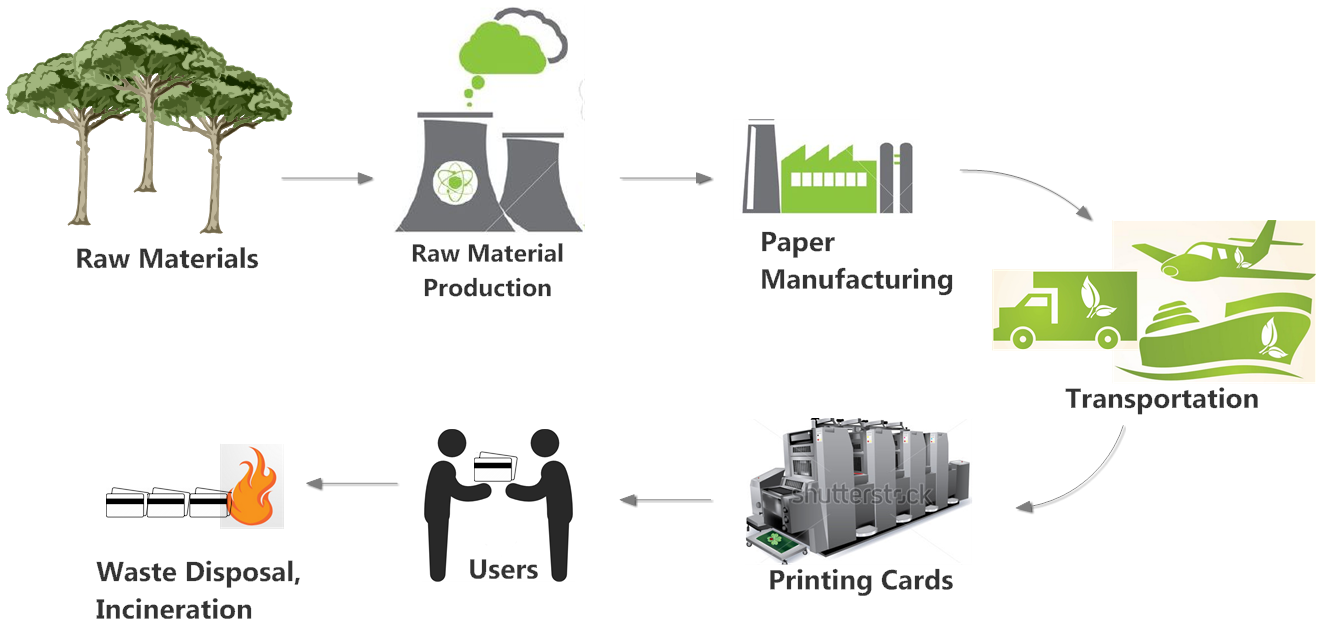
\includegraphics[width=\linewidth]{PBCSystem1.png}
\label{PBCSystem}
\caption{PBC system}\vspace*{-6pt}
\endminipage\hfill
\minipage{0.40\textwidth}
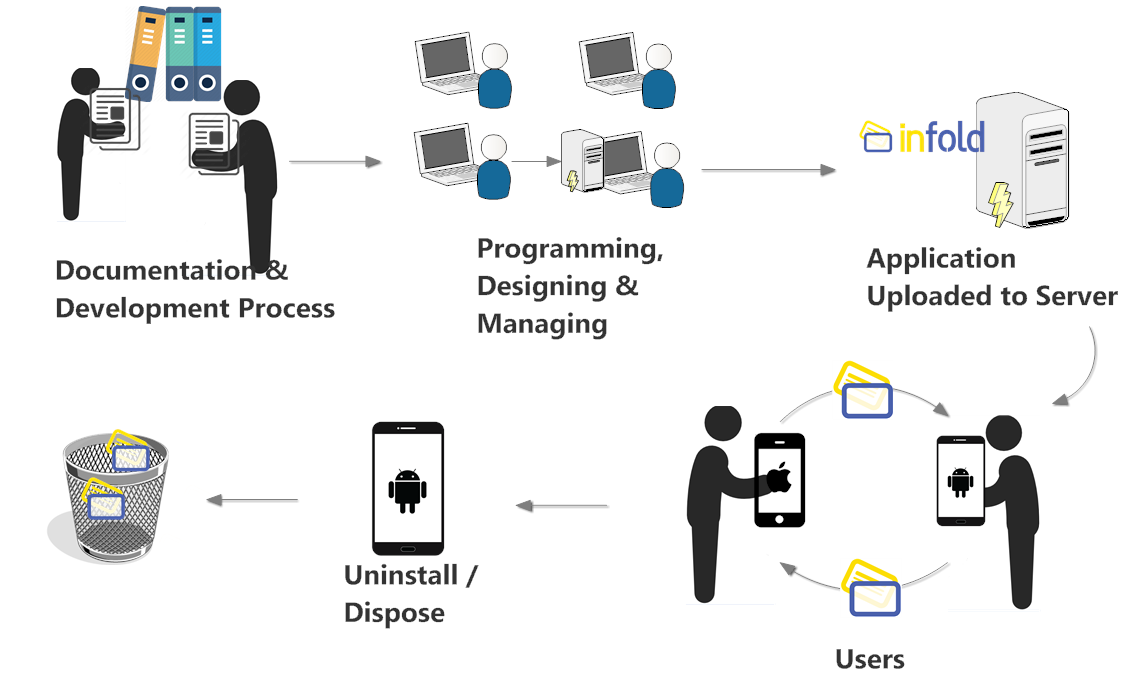
\includegraphics[width=\linewidth]{DBCSystem.png}
\label{DBCSystem}
\caption{DBC system}\vspace*{-6pt}
\endminipage\hfill
\end{figure}
\end{comment}

\section{Methodology}

We model separately the life cycles of PBC and DBC systems in a two-stage cradle-to-grave LCA for evaluating their life cycle impacts as well as total energy consumption, GHG emissions and toxic releases. The first stage (screening analysis) relies on the EIO approach and the second stage is based on the ISO in accordance to ISO 14040 LCA methodology and aims at providing a comprehensive examination and quantification of life cycle impact categories and burdens to validate the findings from the first stage.

\subsection{General Assumptions}\label{Generalassume}
To compare DBC and PBC systems, some general assumptions were required which apply to both stages of this LCA analysis and are detailed below.

\begin{itemize}[]
\item The customer uses PBC or the DBC software for creating and exchanging business cards.
\item Customers exhaust all their printed business cards in one year.
\item The weight of a single PBC was estimated to be 1.8194 g.
\item The DBC software has the same functionality as the PBC system's scope without other options like management, broadcast, copy and translation of business cards.
\item The utilized energy during operation of the DBC software was measured using PowerTutor mobile application\cite{zhang2010accurate} (approximately 0.002778 Wh/exchange). The measured energy usage is an upper bound.
 \item Each DBC has an average size of 10 KB and therefore each exchange between two customers is an exchange of 40 KB data over the Internet which includes the information packet header's size. We assume that 1 MB of traffic across the Internet takes 5.9 Wh which is an upper bound and includes cooling, UPS, wiring, broadband routers, telephone lines \cite{Moshnyaga:2013}. 
\item No DBC software updates are required and therefore we do not account for energy use for their development.
\item The environmental impact from the production of server used in DBC system is considered since it is allocated specifically for the purposes of DBC software.
\item Servers usually have more than one year lifetime, however, the considered production cost of server used in the DBC system is for one year.
 \item The upper-bound server energy consumption for the DBC system was estimated at 45 Wh based on the data from the hosting provider (Digital Ocean).
\item We do not account for the production and manufacturing of smartphones used in DBC system, since they are not utilized specifically for the DBC software and this application constitutes a very minimal and ancillary aspect of their functionality.
\item Due to a highly complex structure and diverse functionality of the Internet, this paper ignores all additional environmental impacts and energy use associated with its components and devices except those allocated specifically for exchanging DBC.
\end{itemize}

\subsection{Functional Unit}\label{sec:FunctionalUnit}

A functional unit defines the foundation of LCA for comparing two or more products. All the data collected in the inventory will be dependent on the defined functional unit. In this study, DBC and PBC products are compared on a one-to-one basis. An exchange of each of them between two customers requires an exchange of two business cards or two equivalent information packets. In order to obtain a comprehensive and accurate picture of DBC and PBC system's life cycle impacts, two cases of functional units were considered; a case of 1000 exchanges between customers in PBC and DBC systems, that is production and exchange of 2000 PBC and DBC respectively and a case of 33000 exchanges between customers in PBC and DBC systems or production and exchange of 66000 PBC and DBC respectively. The latter case is based on data on the annually utilized business cards at Masdar Institute of Science and Technology - a post-graduate university with around 1000 employees (students, faculty, and staff).

\begin{comment}
It is worth mentioning that in DBC system, a customer can broadcast a single information packet representing the business card to other customers which is much more efficient in terms of bandwidth consumption rather than a one-to-one exchange. Even though the latter functionality is energy beneficial to DBC system, but for the unbiased comparison, it is not considered since there is no feasible way to broadcast in PBC system.\\
\end{comment}

\subsection{System Boundaries} \label{PBCBoundary}
Life cycle model of the PBC system is composed of five major stages which, along with their model elements, are listed in Table \ref{PBCboundary}. A PBC is generally composed of paper and ink. These components are acquired from chemical manufacturing and paper manufacturing processes which require natural resources. Paper manufacturing sector is not available in some countries, hence the transportation of paper based products could be included. After obtaining the paper with a suitable quality, thickness and predetermined size, PBC design procedure begins followed by the printing stage. Printed PBC are collected and stored in the appropriate facilities and then delivered to the customers. Then costumers exchange PBC during various events including conferences and meetings. When the useful life of the PBC is expired, the product is disposed as a municipality waste or incinerated.

\begin{table}[h]
\caption{Life cycle model of the PBC system}
\begin{tabular*}{\hsize}{@{\extracolsep{\fill}}lllll@{}}
\toprule
Material Production & Manufacturing  & Distribution & Use & End-of-Life\\
\colrule
Paper Production &  PBC Creation and Printing & Facility Infrastructure & PBC Exchange & PBC Disposal \\
 Ink Production &   & Collection and Storage &  &  \\
 &   & PBC Delivery &  &  \\
\botrule
\end{tabular*}
\label{PBCboundary}
\end{table}
DBC system boundary is quite different from the system boundaries of traditional industrial products. The life cycle model of the DBC system considered in this paper is similar to that of a digital product\cite{Moshnyaga:2013, moshnyaga2013assessment} and along with the model elements is detailed in Table \ref{DBCboundary}. The DBC system has no raw materials as an input to the system. The manufacturing stage of the DBC system involves typical software engineering process, as well as tools and facilities used by the corresponding personnel in charge of the development of the DBC software. The aforementioned facilities and tools include but are not limited to software and equipment like PCs, Air Conditioners, UPSs, printers, and lighting. After the development stage, the DBC software is deployed online so that it is accessible for customers. Once the DBC software is downloaded and installed on a smartphone, a customer starts using the software for creating and exchanging DBC, during which the according information packets are routed through the Internet. Further environmental burdens are associated with the production and disposition of the server. Finally, end-of-life stage is simply uninstalling the DBC software from a smartphone. 


\begin{table}[h]
\caption{Life cycle model of the DBC system}
\begin{tabular*}{\hsize}{@{\extracolsep{\fill}}llll@{}}
\toprule
Manufacturing & Distribution & Use & End-of-Life\\
\colrule
Software Engineering &  DBC Software Installation  & Server Production and Disposal & DBC Software Uninstallation\\
DBC Software Development &   & Smartphone Use  & \\
Facility Infrastructure  &   & File Transfer and DBC Exchange &   \\
\botrule
\end{tabular*}
\label{DBCboundary}
\end{table}
\vspace*{-0.5cm}

\section{Screening Analysis} \label{ScreeningLCA}

We do a screening of the environmental impacts and energy consumption of PBC and DBC systems using Carnegie Mellon EIO LCA tool, based on U.S. data from 2002 \cite{Mellon}. The monetary expenses were calculated for DBC and PBC systems in both cases of functional units and served as an input to EIO LCA. The calculations for the DBC system shown in Table \ref{PBCcalc} are based on the assumption that electricity price is 0.2 USD per KWh (based on statistics on the electricity price in U.S.). For the PBC system's calculations it was assumed that the average cost of printing 200 standard business cards is 50 USD. This assumption derived from the extensive observations on the price statistics offered by various U.S. based business card printing services.

\begin{table}[h]
\label{PBCcalc}
\caption{Monetary expenses of the DBC system}
\begin{tabular*}{\hsize}{@{\extracolsep{\fill}}ll@{}}
\colrule
\textbf{Production of a server} & 240 USD annually \\
\textbf{Production of a software}  &   8000 USD \\
(all inclusive cost considering expenses associated with the corresponding personnel and facilities) &  \\
\textbf{Total energy consumption} (software installation + smartphone + server) &  394.439 KWh hence, associated \\
(for 1000 exchanges) & expenses are 78.88 USD \\
\textbf{Total energy consumption} (software installation + smartphone + server) & 406.1389 KWh hence, associated  \\
(for the case of 33000 exchanges) & expenses are 81.227 USD  \\
\botrule
\end{tabular*}
\end{table}

The environmental impacts and energy consumption of PBC and DBC systems for both cases of functional units i.e. 1000 and 33000 exchanges are presented in Figure \ref{screen1}, Figure \ref{screecn3Sectors} and Figure \ref{screecn4Sectors}. The toxic releases shown in Figure \ref{screen1} refer to different environments such as surface and under water, land, air and include metals and non metals. Economic sectors that have less than 1\% contribution to the aggregate GHG emissions are represented in a single compound sector entitled "Other sectors" in Figure \ref{screecn3Sectors} and Figure \ref{screecn4Sectors}. For the case of 1000 exchanges Figure \ref{screen1} shows that the PBC system has less environmental impact and energy consumption compared to the DBC system for the small scale application and is reversed for the large-scale one. For the case of 33000 exchanges the DBC system is far more environmentally friendly than the PBC system emitting almost 3 times less GHGs. Likewise, the PBC system's energy and toxic releases are nearly 4 and 10 times higher than those of the DBC system respectively. The results shown in Figure \ref{screecn3Sectors} indicate that GHG emissions of the PBC system are mainly driven by two sectors, namely power generation and supply (38\%) and paper mills (15\%), followed by truck transportation (5\%), oil and gas extraction (5\%) and printing (5\%) sectors having relatively small impacts. This implies that the large portion of the GHG emissions of the PBC system are due to the electricity usage and paper production during the manufacturing and material production life cycle stages. Unlike the PBC system, where GHG emissions are more or less evenly distributed among the sectors the dominating GHG emitting sector in the DBC system is power generation and supply, which demands 85\% of the cumulative GHG emissions as shown in Figure \ref{screecn4Sectors}. Hence, it could be concluded that GHG emissions from electricity consumption and server equipment production during the manufacturing and use stages of the DBC system life cycle significantly affect its GHG emissions and a higher RE penetration can directly reduce total emissions. 
\begin{figure}[t]
\minipage{0.52\textwidth}
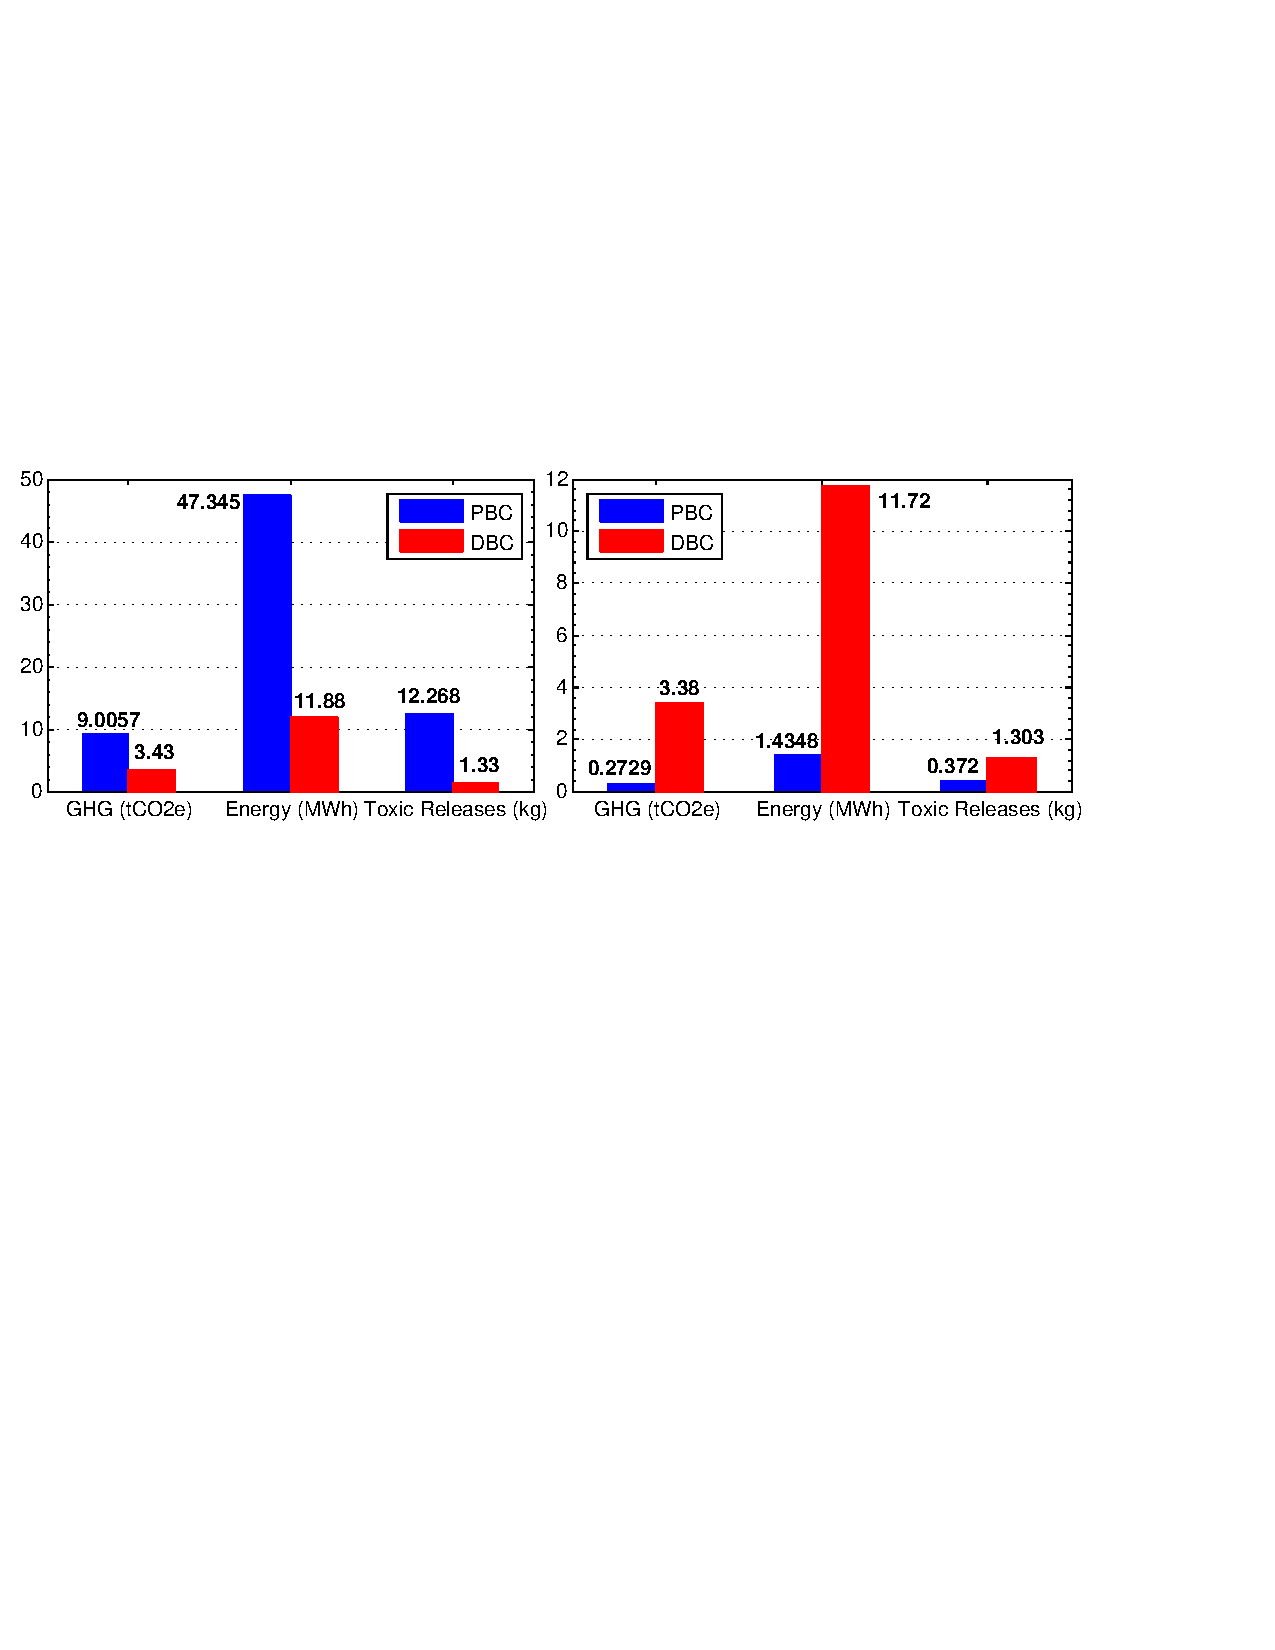
\includegraphics[width=\linewidth]{sf.pdf}
\caption{Screening of life cycle burdens of PBC and DBC systems for 1000 and 33000 exchanges on right and left respectively}
\label{screen1}
\endminipage\hfill
\minipage{0.42\textwidth}
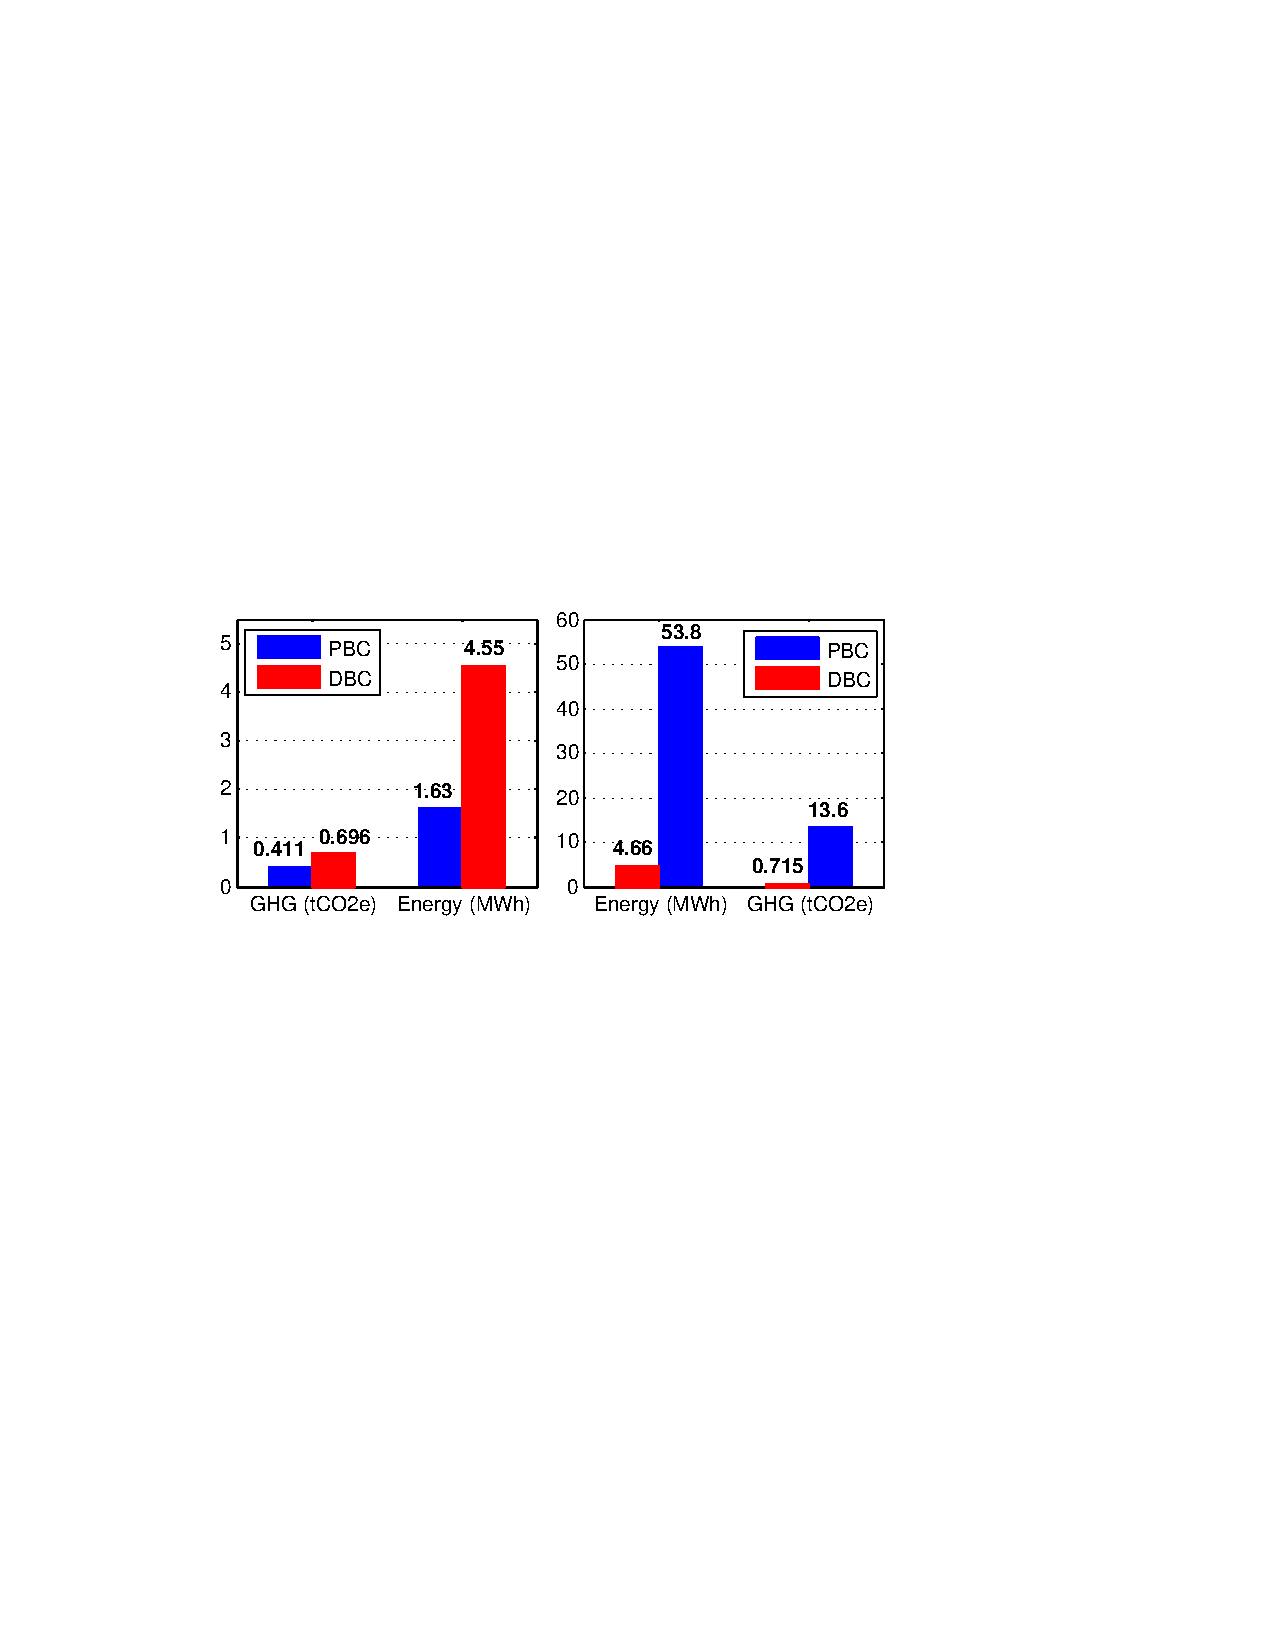
\includegraphics[width=\linewidth]{fs.pdf}
\caption{Second stage analysis of life cycle impacts of PBC and DBC systems for 1000 and 33000 exchanges of on left and right respectively}
\label{fig:onescore}
\endminipage\hfill
\end{figure}
\begin{figure}[t]
\minipage{0.49\textwidth}
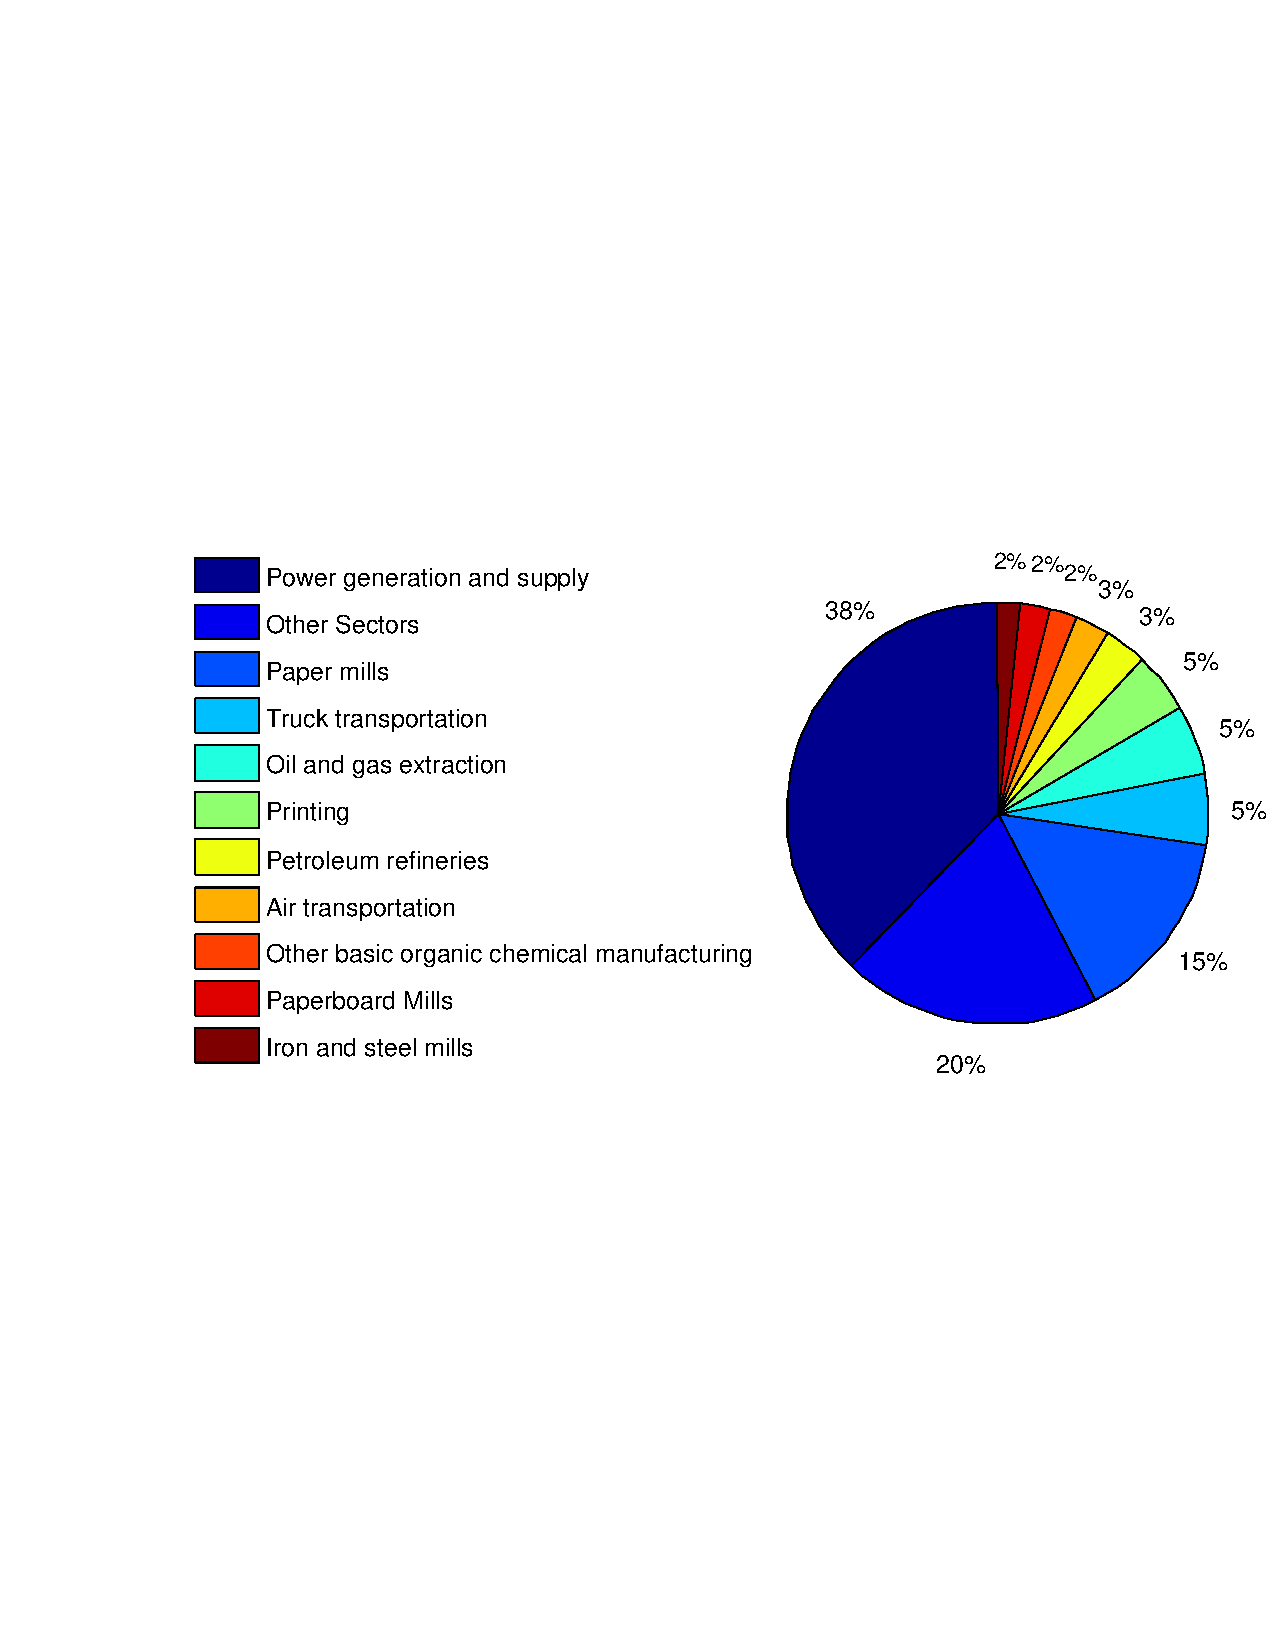
\includegraphics[width=\linewidth]{f.pdf}
\caption{Screening of GHG emissions of the PBC system by economic sectors}
\label{screecn3Sectors}
\endminipage\hfill
\minipage{0.43\textwidth}
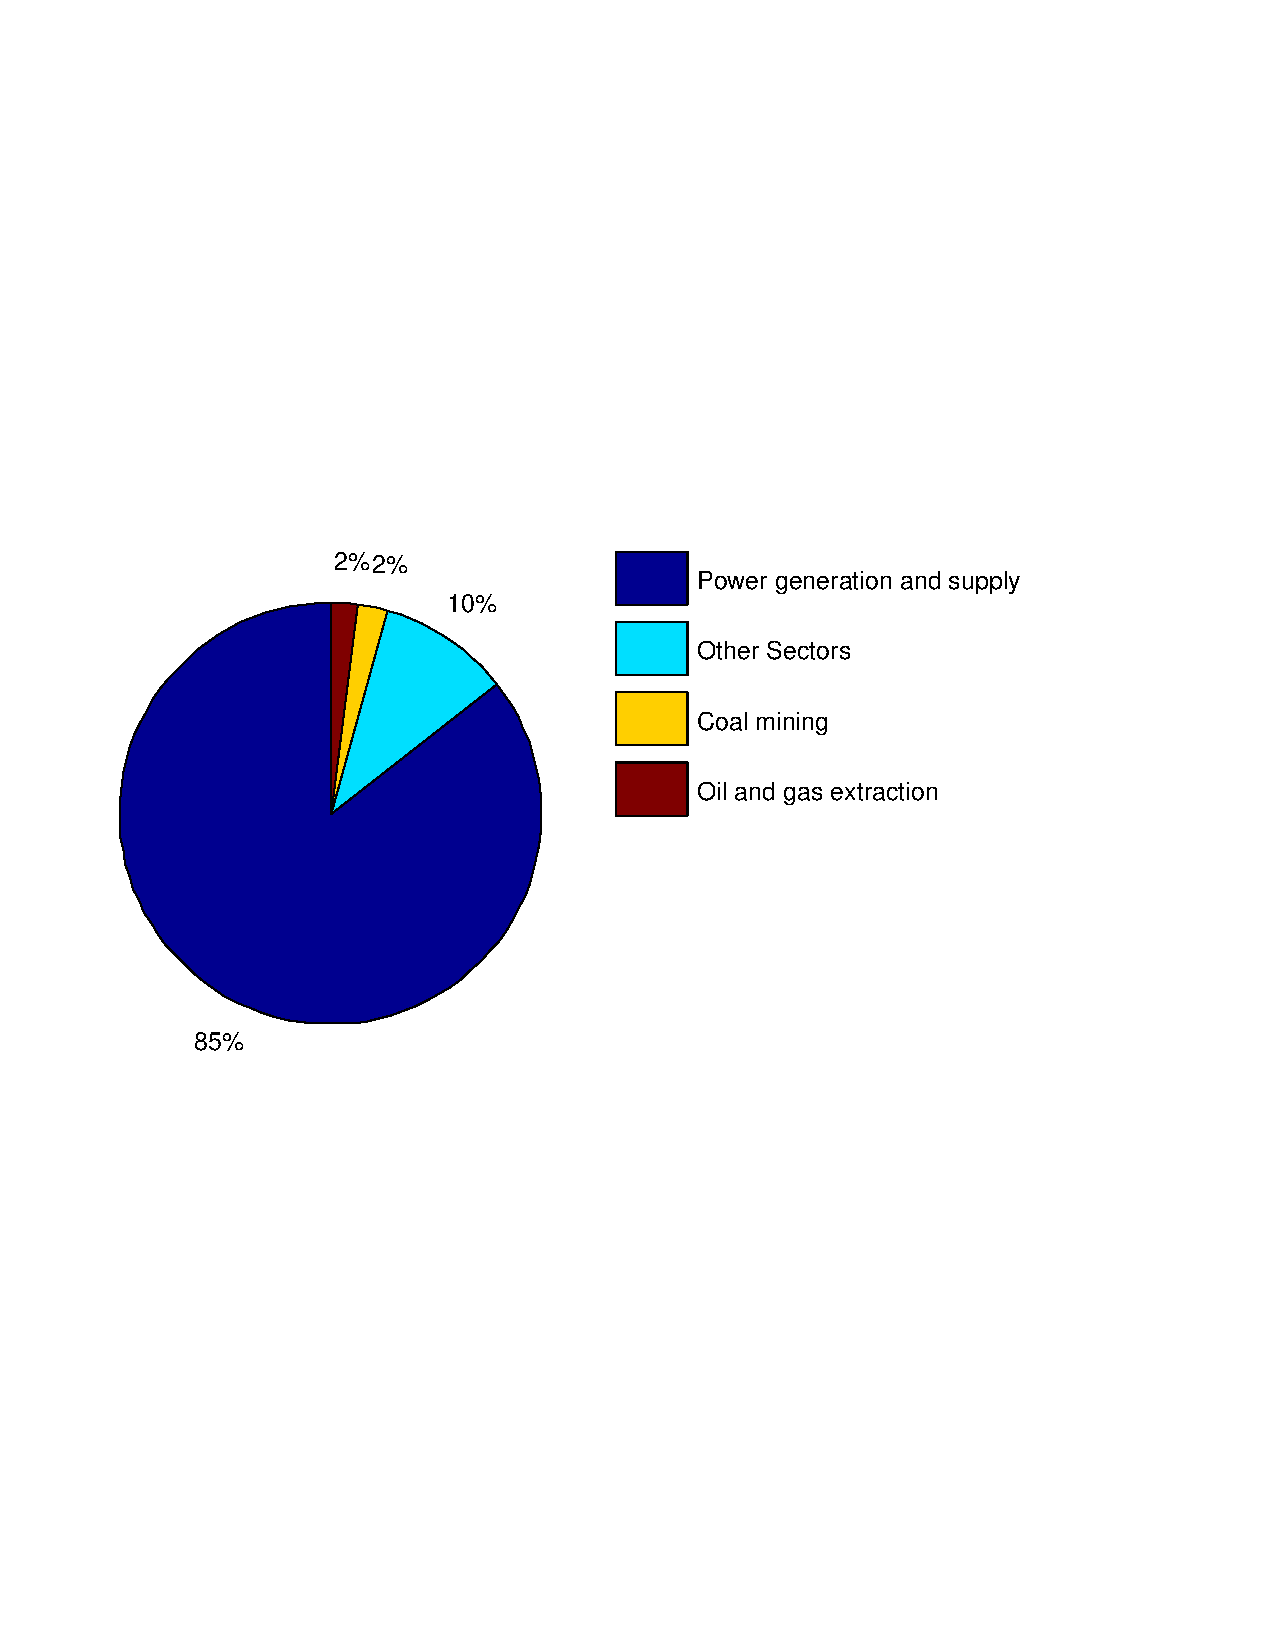
\includegraphics[width=\linewidth]{g.pdf}
\caption{Screening of GHG emissions of the DBC system by economic sectors}
\label{screecn4Sectors}
\endminipage\hfill
\end{figure}

\section{Second Stage Analysis}
An in-depth analysis and quantification of environmental impact categories and life cycle burdens has been conducted for the second stage of this LCA analysis using SimaPro 7.3 software with EcoInvent 3.1 database based on U.S. data from 2004.

\subsection{Life Cycle Inventory}

Data collection and calculations performed in the Life Cycle Inventory (LCI) phase of this study, which quantify associated inputs and outputs in the PBC and DBC systems are provided previously in subsection \ref{Generalassume}.\\

LCI results for the PBC and DBC systems for both cases of functional units are shown in Figure \ref{fig:onescore}. For brevity life cycle impacts other than GHG emissions and energy consumption are not discussed. The results confirm the screening analysis but narrow the difference in the small scale and increase it in the large scale. For the case of the functional unit being 1000 exchanges the DBC system emitted only about 1.7 times the amount of CO2 equivalent emissions than the PBC system. Likewise, the energy consumption of the DBC system at 4.55 MWh is only three times higher than the energy demand of the PBC system. Moreover, for the case of 33000 exchanges, the difference between LCI and EIO LCA results are more noticeable as could be seen from Figure \ref{fig:onescore}. The difference between results may imply the following: (1) life cycle burdens of the DBC system largely depend on the fixed impact which is nothing else but the burdens caused by development of the DBC software and manufacturing of server hardware (2) life cycle impacts of the PBC system heavily depend on the number of exchanges (3) the scale economies of the PBC system are remarkably lower than that of the DBC system.

\begin{table}[h]
\caption{Environmental impacts of PBC and DBC systems for 1000 and 33000 exchanges}
\begin{tabular*}{\hsize}{@{\extracolsep{\fill}}llllll@{}}
\toprule
\multicolumn{2}{l}{\multirow{2}{*}{\textbf{}}} & \multicolumn{2}{l}{\textbf{1000 Exchnages}} & \multicolumn{2}{l}{\textbf{33000 Exchanges}} \\ 
\colrule
\multicolumn{2}{l}{} & \textbf{DBC} & \textbf{PBC} & \textbf{DBC} & \textbf{PBC} \\
\multicolumn{2}{l}{\it{Total}} & \it{0.317} & \it{0.279} & \it{0.326} & \it{9.21} \\ 
\multicolumn{2}{l}{Carcinogens} & 0.00106 & 0.00816 & 0.00108 & 0.0269 \\ 
\multicolumn{2}{l}{Non-carcinogens} & 0.00886 & 0.0751 & 0.00909 & 2.48 \\ 
\multicolumn{2}{l}{Respiratory inorganics} & 0.108 & 0.0713 & 0.111 & 2.35 \\
\multicolumn{2}{l}{Ionizing radiation} & 0.00308 & 0 & 0.00317 & 0 \\
\multicolumn{2}{l}{Ozone layer depletion} & 4.60E-05 & 2.11E-04 & 4.80E-05 & 0.00697 \\ 
\multicolumn{2}{l}{Respiratory organics} & 5.27E-05 & 0.000294 & 5.80E-05 & 9.72E-03 \\
\multicolumn{2}{l}{Aquatic ecotoxicity} & 0.00748 & 0.000651 & 0.00769 & 2.15E-02 \\
\multicolumn{2}{l}{Terrestrial ecotoxicity} & 0.00684 & 0.0401 & 0.00701 & 1.32 \\ 
\multicolumn{2}{l}{Terrestrial acidification} & 0.00127 & 0.00089 & 0.00131 & 0.0294 \\ 
\multicolumn{2}{l}{Land occupation} & 0.00204 & 0.00229 & 0.0021 & 0.0756 \\ 
\multicolumn{2}{l}{Global warming} & 0.0703 & 0.0415 & 0.07222 & 1.37 \\ 
\multicolumn{2}{l}{Non-renewable energy} & 0.108 & 0.0387 & 0.111 & 1.28 \\ 
\multicolumn{2}{l}{Mineral extraction} & 2.89E-04 & 0.000001918 & 2.96E-04 & 6.33E-05 \\ 

\botrule
\end{tabular*}
\label{PBCandDBCexchanges}
\end{table}

\subsection{Life Cycle Impact Assessment}
Life Cycle Impact Assessment (LCIA) phase of this LCA study focuses on revealing and assessing environmental impacts and impact categories of PBC and DBC systems throughout their life cycle. LCIA results presented in Table \ref{PBCandDBCexchanges} represent a single score comparison between both systems based on the conversion of LCI results to weighted units.\\

For the case of the functional unit being 1000 exchanges, environmental impact of the PBC system is slightly lower than that of the DBC system as could be seen from Table \ref{PBCandDBCexchanges}. Specifically, the DBC system emitted nearly two times higher quantities of global warming emissions and chemicals  related to acidification than the PBC system. In addition the DBC system emitted nearly twenty times higher ozone depleting substances that the PBC system. Whereas, when it comes to raw materials the PBC system required almost 10 times higher amount of raw materials than the DBC system. These can be explained by the initial high impacts posed by the manufacturing and use stages of the DBC system life cycle. On the contrary, the DBC system is preferable when the functional unit is 33000 exchanges, with the overall environmental impact of the PBC system being about 30 times higher than that of the DBC system. Furthermore, the PBC system has far worse impacts in almost all environmental categories than the DBC system. This is because the manufacturing and use stages of the DBC system life cycle have been amortized over high number of exchanges. Considering the findings from both stages of this LCA analysis, it is safe to assume that up to certain limit the higher the number of exchanges, the more amortized are the impacts caused by the manufacturing and use stages of the DBC system life cycle.

\section{Conclusions}

In this paper the findings of a comparative life cycle assessment of paper-based and software-based business card systems are presented. For reliable and accurate results, two-stage cradle-to-grave analysis of environmental impacts and impact categories of the two systems is conducted for two cases of functional units. In addition, energy consumption, GHG emissions and toxic releases of the two systems have been analyzed and quantified. Under the considered assumptions, for the case of a small scale functional unit the paper-based business card system is more environmentally friendly and economical in terms of energy consumption. Nevertheless, for the case of a large scale (real world scenario) functional unit the software-based business card system has significantly less environmental impact and energy utilization compared to the paper-based system. The results indicate that life cycle burdens of the software-based business card system are mainly driven from
the electricity consumption and server equipment production
during the manufacturing and use stages of its life cycle. Similarly, electricity usage and paper production during the manufacturing and material production life cycle stages of the paper-based business card system are the major contributors to its life cycle impacts. Sensitivity analysis of the results is a subject to future work. This study is not meant to label or discourage paper-based or software-based business cards. Instead, the findings of this study provide industry and consumers with adequate information for considering environmentally aware decisions
regarding the two systems. Furthermore, this paper contains information regarding software life cycle assessment that could be useful for the development of sustainable technologies and green software. 

\begin{comment}
\section*{Acknowledgment}

This study was conducted under the support and funding of Masdar Institute of Science and Technology.
\end{comment}

\bibliography{reference}
\bibliographystyle{model3a-num-names}

\end{document}

%%
%% End of file `procs-template.tex'.
